\documentclass{sprawozdanie-agh}

\usepackage[utf8]{inputenc}
\usepackage{listings}
\usepackage{xcolor}
\usepackage{graphicx}
\usepackage{caption}
\usepackage{graphicx}
\usepackage{lipsum}
\usepackage{wrapfig}
\usepackage{subcaption}
\usepackage{accsupp}
\usepackage{array}
\usepackage{multirow}
\usepackage{amsmath, siunitx}    
\graphicspath{ {./img/} }
\makeatletter

\begin{document}

\przedmiot{Algorytmy geometryczne}
\tytul{Laboratorium 4}
\podtytul{Przecinanie się odcinków}
\kierunek{Informatyka}
\autor{Kyrylo Iakymenko}
\data{Kraków, 5 grudnia 2023}

\stronatytulowa{}

\section{Wprowadzenie}
\subsection{Cel ćwiczenia}
\quad To ćwiczenie ma na celu zapoznanie się z metodami generacji 
losowych punktów oraz badanie metod klasyfikacji położenia punktów na płaszczyźnie 
względem prostej. 
\subsection{Położenie punktu względem prostej}

\quad Położenie punktu względem prostej będziemy wyznaczać obliczjąc
dane wyznaczniki. Wyznaczniki pozwalają określić położenie
punktu c względem prostej która jest wyznaczona przez punkty a i b.
Jeżeli wyznacznik jest większy od 0 to punkt znajduje się z lewej strony prostej, jeżeli jest mniejszy
od 0  to
punkt znajduje się po prawej stronie prostej, a jeżeli wartość wyznacznika
jest równa 0 (lub jej wartość bezwzględna $< \varepsilon$) to punkt leży na prostej.

\quad Pomimo, że
powyższe wyznaczniki są sobie równoważne to na skutek
niedoskonałości reprezentacji liczb rzeczywistych w komputerze wyniki
mogą się różnić w zależności od użytego wyznacznika.

$$
(1)\det(a, b, c)= \begin{vmatrix}
       a_{x} - c_{x} & a_{y} - c_{y} \\
       b_{x} - c_{x} & b_{y} - c_{y} 
              \end{vmatrix}.\\
              $$
              $$
(2)\det(a, b, c) = \begin{vmatrix}
    a_x & a_y & 1\\
    b_x & b_y & 1\\
    c_x & c_y & 1
\end{vmatrix}.\\
$$

\section{Zbiory testowe}
\subsection{Wykorzystane algorytmy}
\quad W danym ćwiczeniu testujemy działanie następujących algorytmów:
\begin{itemize}
    \item Algorytm sprawdzenia monotoniczności wielokąta względem osi $OY$.
    \item Algorytm klasyfikacji wierzchołków wielokąta ze względu na położenie jego sąsiedzi.
    \item Algorytm triangulacji wielokąta monotonicznego.
\end{itemize}
\subsection{Zbiory testowe}
\quad Na potrzeby ćwiczenia stworzyliśmy 6 wielokątów.
Zostały wybrane odpowiednio, żeby przetestować działanie algorytmów w przypadkach zarówno lososwych jak i ekstremalnych.
\quad Na potrzeby ćwiczenia wygenerujemy $4$ zbiory punktów losowych.
\begin{enumerate}
    \item $10^5$ losowych punktów $(x, y)$ w przestrzeni $\mathbb{R}^2$, gdzie $(x, y) \in \left[-1000,1000\right]^{2}$.
    \item $10^5$ losowych punktów $(x, y)$ w przestrzeni $\mathbb{R}^2$, gdzie $(x, y) \in \left[-10^{14},10^{14}\right]^{2}$.
    \item $1000$ losowych punktów w przestrzeni $\mathbb{R}^2$ leżących na okręgu o środku $ O = (0,0)$ i promieniu $ R = 100$.
    \item $ 1000$ losowych punktów w przestrzeni $\mathbb{R}^2$ dla $ x \in \langle -1000,1000 \rangle$ leżących na prostej wyznaczonej przez wektor $ \overrightarrow{ab}$.   
    Gdzie $ a = (-1.0, 0.0)$, $ b = (1.0, 0.1)$.
\end{enumerate}

\section{Algorytm zamiatania}
\quad Algorytm zamiatania (ang. sweep line algorithm) to efektywna metoda rozwiązania problemu wyznaczania przecięcia się odcinków na płaszczyźnie. Algorytm ten można opisać w kilku krokach:


\begin{enumerate}
    \item 
    \textbf{Sortowanie punktów końcowych odcinków:}
    Algorytm rozpoczyna się od posortowania punktów końcowych odcinków według współrzędnej x. Dzięki temu możemy ustalić kolejność, w jakiej algorytm będzie przetwarzał odcinki.
    
    \item  \textbf{Sweepline:}
Algorytm używa 'miotły', która przesuwa się przez posortowane punkty. Linia ta reprezentuje aktualne położenie algorytmu na płaszczyźnie.

\item  \textbf{Struktura danych do przechowywania aktywnych odcinków:}
Tworzona jest struktura danych, najczęściej używane to drzewo binarne przeszukiwań lub struktura zrównoważona, które przechowuje aktualnie przecinane przez sweepline odcinki.

\item  \textbf{Przeszukiwanie sweepline:}
Sweepline przemieszcza się przez posortowane punkty, a w miarę tego ruchu algorytm aktualizuje strukturę danych, śledząc, które odcinki są obecnie przecinane przez sweepline.

\item  \textbf{Znajdowanie przecięć:}
Przy każdym ruchu sweepline, algorytm sprawdza, czy doszło do przecięcia pomiędzy aktualnym odcinkiem, a innymi odcinkami znajdującymi się nad lub pod sweepline. W przypadku wykrycia przecięcia, jest ono rejestrowane.

\item  \textbf{Obsługa przypadków szczególnych:}
Algorytm uwzględnia różne przypadki przecięć, takie jak przecięcia proste, styczne, czy nakładające się odcinki. Obsługuje również sytuacje szczególne, takie jak wspólne punkty i brzegi odcinków.

\item  \textbf{Aktualizacja struktury danych:}
W miarę poruszania się sweepline, struktura danych jest aktualizowana, a odcinki, które już zostały przetworzone, są usuwane z niej.

\end{enumerate}

Algorytm zamiatania jest stosunkowo prosty do zrozumienia i implementacji, a jego złożoność czasowa wynosi $O(n log n)$, gdzie n to liczba odcinków. Działa efektywnie, zwłaszcza w przypadku dużych zbiorów danych, co czyni go popularnym narzędziem w problemach związanych z geometrią obliczeniową.









% \newpage
\section{Wyniki algorytmu}
\begin{figure}[!h]
    \centering
    \begin{subfigure}{.5\textwidth}
      \centering
      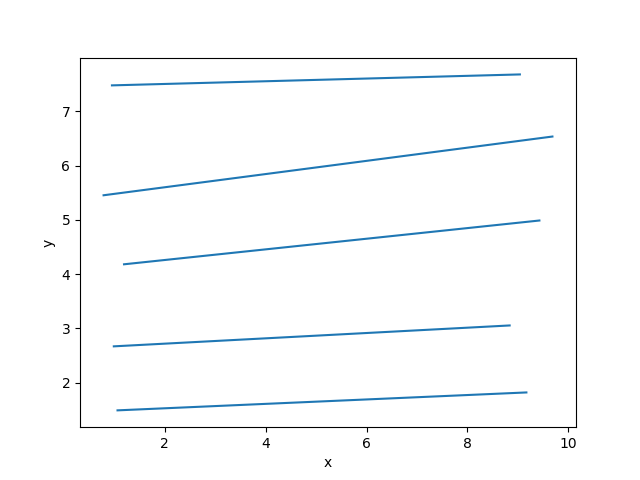
\includegraphics[width=.9\linewidth]{0_int.png}
      \caption*{Rys. 7}
      \label{fig:sub1}
    \end{subfigure}%
    \begin{subfigure}{.5\textwidth}
      \centering
      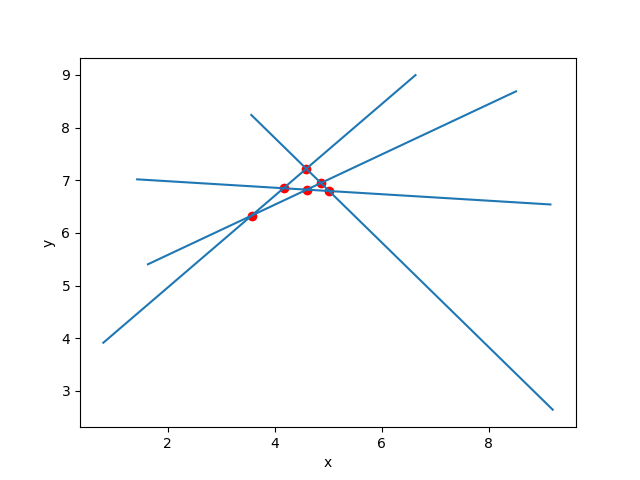
\includegraphics[width=.9\linewidth]{1_int.png}
      \caption*{Rys. 8}
      \label{fig:sub2}
    \end{subfigure}
    \label{fig:test}
    \end{figure}

% \newpage

    \begin{figure}[!h]
    \centering
    \begin{minipage}{.5\textwidth}
      \centering
      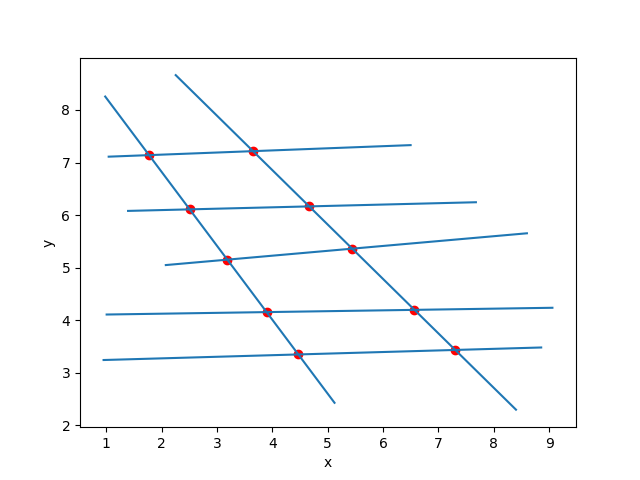
\includegraphics[width=.9\linewidth]{2_int.png}
      \caption*{Rys. 9}
      \label{fig:test1}
    \end{minipage}%
    \begin{minipage}{.5\textwidth}
      \centering
      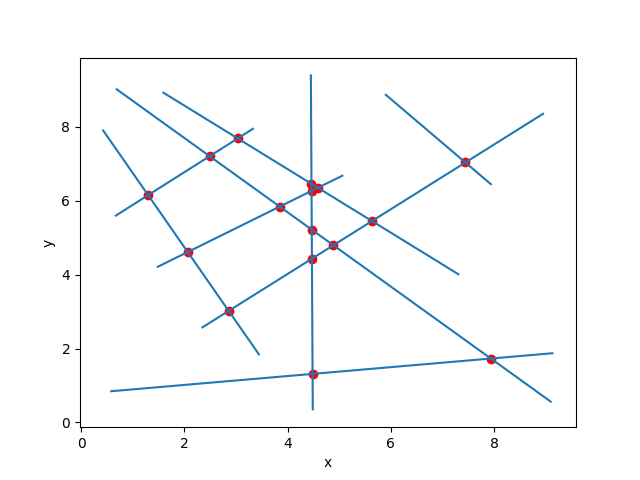
\includegraphics[width=.9\linewidth]{3_int.png}
      \caption*{Rys. 10}
      \label{fig:test2}
    \end{minipage}
    \end{figure}
    \begin{figure}[!h]
        \centering
        \begin{minipage}{.5\textwidth}
          \centering
          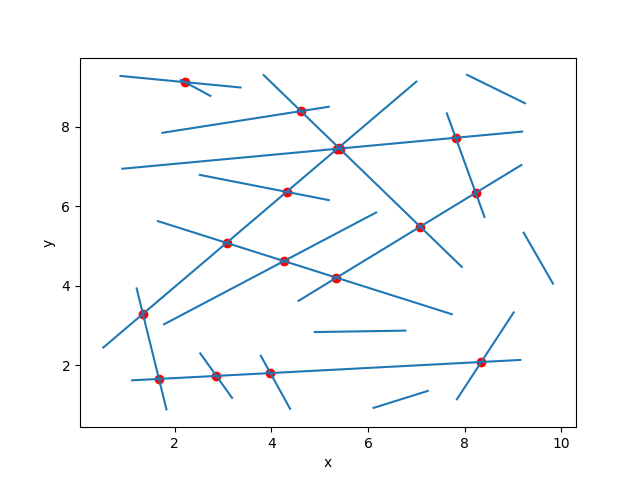
\includegraphics[width=.9\linewidth]{4_int.png}
          \caption*{Rys. 11}
          \label{fig:test1}
        \end{minipage}%
        \begin{minipage}{.5\textwidth}
          \centering
          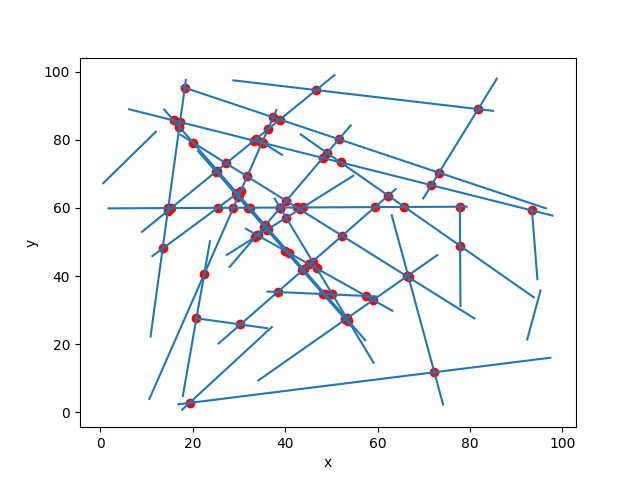
\includegraphics[width=.9\linewidth]{5_int.png}
          \caption*{Rys. 12}
          \label{fig:test2}
        \end{minipage}
        \end{figure}
\section{Podsumowanie}
\quad 
Skuteczność Algorytmu:
Algorytm zamiatania wykazuje się wysoką skutecznością w identyfikowaniu przecięć odcinków na płaszczyźnie. Jego zdolność do obsługi różnych przypadków przecięć, takich jak przecięcia proste, styczne czy nakładające się odcinki, sprawia, że jest on wszechstronnym narzędziem do rozwiązania problemów geometrii obliczeniowej związanego z odcinkami.

Złożoność Obliczeniowa:
Warto zauważyć, że algorytm zamiatania ma relatywnie niską złożoność obliczeniową w porównaniu do niektórych innych metod wyznaczania przecięć odcinków. Jego efektywność staje się szczególnie istotna w przypadku dużej liczby odcinków, gdzie inne podejścia mogą być bardziej kosztowne obliczeniowo.

Przydatność w Praktyce:
Algorytm zamiatania znajduje zastosowanie w wielu praktycznych dziedzinach, takich jak grafika komputerowa, planowanie tras czy analiza obrazów medycznych. Jego prostota implementacyjna i skuteczność czynią go atrakcyjnym narzędziem dla programistów i badaczy zajmujących się problemami geometrii obliczeniowej.

Obsługa Sytuacji Wyjątkowych:
Omawiane sprawozdanie uwzględnia obsługę różnych przypadków szczególnych, takich jak wspólne punkty i brzegi odcinków. To potwierdza, że algorytm zamiatania jest elastyczny i potrafi radzić sobie z różnorodnymi sytuacjami, co zwiększa jego użyteczność w praktyce.

Wyzwania Implementacyjne:
Pomimo ogólnej efektywności, implementacja algorytmu zamiatania może wymagać uwzględnienia wielu szczegółów. W przypadku bardziej skomplikowanych scenariuszy, programiści powinni być świadomi potencjalnych wyzwań związanych z obsługą sytuacji granicznych i optymalizacją kodu.

Jedną ze zmian, którą trzeba było zrealizować było zwracanie w wyniku triangulacji, zarówno oryginalnego 
wielokąta jak i triangulacji po indeksach. To pozwala na wygodny odczyt tej struktury i możliwości szybkiej wizualizacji wyników. Także 
ten sposób przechowywania wyniku algorytmu uniemożliwia błędy związane ze złym dopasowaniem triangulacji do właściwego wielokąta, gdyż zarówno wielokąt, jak i wynik są przechowywane razem. 
Jeszcze jedną rzeczą na którą trzeba było zwrócić uwagę była reprezentacja triangulacji jako listy par indeksów wierzchołków, zamiast listy par współrzędnych wierzchołków. 
To pozwala przede wszystkim na zmiejszenie ilości używanej pamięci, ale również jest bardziej eleganckim rowiązaniem, które upraszcza implementacje algorytmu.
\end{document}